% ===========================================================================
% Draft manuscript -- Multimodal Lunar Benchmark
% Every table is generated by `python -m src.experiments.make_tables` and
% included below; do not type results by hand.  \TODO{} marks items that need
% an author decision or a verified citation.
% ===========================================================================
\documentclass[10pt]{article}
\usepackage[margin=1in]{geometry}
\usepackage{booktabs,graphicx,amsmath,hyperref,float}
\newcommand{\TODO}[1]{\textbf{[TODO: #1]}}
\graphicspath{{../figures/}}

\title{A Region-Held-Out Multimodal Benchmark for Lunar Optical, Elevation and Thermal Data}
\author{\TODO{authors}}
\date{}

\begin{document}
\maketitle

\begin{abstract}
Learning across lunar remote-sensing modalities is hindered by the lack of a
shared, pixel-aligned benchmark with defensible evaluation protocols. We
release a benchmark of 28 regions (448 tiles of $64\times64$ pixels) that
co-registers LROC WAC optical imagery, LOLA elevation and Diviner midnight
bolometric temperature on a common 128~px/deg grid, with derived slope and
hillshade layers and per-pixel validity masks. Regions span both hemispheres,
nearside and farside, and mare, highland, young-crater, rille and landing-site
terrain. We define two tasks, a region-level train/validation/test split that
holds out a southern young crater and a farside crater, and baselines ranging
from a train-mean predictor to a small CNN, reporting both absolute error and a
tile-demeaned ``anomaly'' $R^2$ that isolates spatial structure.
A small CNN lowers held-out thermal RMSE from 7.6~K (train mean) to 5.8~K and
optical-only slope RMSE from $6.8^\circ$ to $4.2^\circ$, yet no learned thermal
baseline recovers within-tile structure on unseen regions (anomaly $R^2<0$),
leaving a clear open problem.
\end{abstract}

\section{Introduction}
The Lunar Reconnaissance Orbiter has produced complementary global views of the
Moon: optical imagery from the LROC Wide Angle Camera \cite{robinson2010lroc},
topography from the Lunar Orbiter Laser Altimeter (LOLA)
\cite{smith2010lola,smith2017lola} and surface temperatures from the Diviner
Lunar Radiometer \cite{paige2010diviner,williams2017diviner}. These products
differ in resolution, projection, tiling and acquisition geometry, so a
learning problem that spans modalities first requires a careful, shared
georeferenced grid. Machine learning on the Moon has so far largely addressed
single-modality problems such as crater identification from topography
\cite{silburt2019deepmoon}, while Earth observation already benefits from
large aligned benchmark archives \cite{sumbul2019bigearthnet,schmitt2019sen12ms}.
This paper provides the corresponding resource for the Moon: a pixel-aligned,
masked, region-split benchmark of optical, elevation and thermal data.
Our contributions are: (i) a reproducible pipeline that builds aligned
multimodal tiles from public PDS products using HTTP range requests and
requires no multi-gigabyte downloads for LOLA or Diviner; (ii) a 28-region
benchmark with explicit validity masks; (iii) region-held-out splits and tasks
with strong yet simple baselines, including a latitude-only reference;
(iv) an honest account of alignment quality and dataset limitations.

\section{Related Work}
\paragraph{Lunar instruments and data products.}
The three modalities we combine come from LRO instruments with published
overviews: LROC \cite{robinson2010lroc}, LOLA \cite{smith2010lola,smith2017lola}
and Diviner \cite{paige2010diviner,williams2017diviner}. We reuse their public
PDS products and contribute the harmonization, masks and evaluation protocol
rather than new measurements.
\paragraph{Learning from lunar data.}
DeepMoon \cite{silburt2019deepmoon} shows that convolutional networks can
identify craters from lunar topography; this is a single-modality task.
\paragraph{Remote-sensing benchmarks.}
Earth observation has aligned, curated archives such as BigEarthNet
\cite{sumbul2019bigearthnet} and SEN12MS \cite{schmitt2019sen12ms}, and
dataset-and-challenge efforts such as fMoW \cite{christie2018fmow} and SpaceNet
\cite{vanetten2018spacenet}. Our benchmark follows the same spirit for the
Moon, with explicit validity masks and region-level splits.
\TODO{authors to confirm novelty: we are not aware of a public, pixel-aligned
optical--elevation--thermal lunar benchmark with region-held-out evaluation,
but this paper does not rest on an exhaustive survey; add any missed prior work.}

\section{Data and Construction}
\paragraph{Sources.}
WAC 100~m global morphology mosaic \cite{robinson2010lroc} (nodata~$=0$), LOLA
LDEM\_256 \cite{smith2010lola} (256~px/deg, height in km relative to a
1737.4~km sphere) and the Diviner TBOL\_SAM midnight map
\cite{paige2010diviner,williams2017diviner} (128~px/deg, $70^\circ$S--$70^\circ$N).
All products are NASA PDS.
\paragraph{Common grid.}
Equirectangular, sphere radius 1{,}737{,}400~m, 128~px/deg ($\approx$236.9~m).
Each region is a $2^\circ\times2^\circ$ box ($256\times256$~px) cut into 16
non-overlapping $64\times64$ tiles. Diviner is already on this grid (pixel
centres are verified equal); LOLA is aggregated by an exact $2\times2$ block
mean; WAC is area-averaged with a coverage layer recording the fraction of
non-nodata source pixels per cell.
\paragraph{Derived layers and masks.}
Slope and hillshade are computed from the common-grid DEM
(central differences via \texttt{numpy.gradient} with latitude-dependent
east--west pixel spacing; hillshade uses sun azimuth 315$^\circ$ and altitude
45$^\circ$). Isolated NaN pixels are nearest-filled and flagged invalid in
the mask/coverage layers.
\paragraph{Supplementary diurnal curve.}
The pixel-level thermal layer is one local time. To add day/night context we
attach to every tile the Diviner bolometric temperature as a function of local
time (96 bins of 0.25~h) from the PDS global cumulative products
\cite{williams2017diviner}, binned at $0.5^\circ\times0.5^\circ$; one bin is
exactly one $64\times64$ tile. This is a tile-level value ($\sim$15~km), not a
pixel-aligned map, and it is not used by any baseline. All 448 tiles have a
midnight value and a noon (11--13~h) value (median noon 379~K, range
315--394~K). As a consistency check, the midnight value agrees with the mean of
our TBOL\_SAM thermal layer over the same tile with correlation 0.993 and RMSE
1.15~K (the cumulative product is 0.73~K warmer on average; it is not
slope-adjusted and covers a different time span).
\paragraph{Regions.}
Table~\ref{tab:regions} lists all regions; Fig.~\ref{fig:montage} shows the
aligned layers.
\begin{table}[H]\centering\scriptsize
\begin{tabular}{llrrllrrrr}
\toprule
region & terrain & lat\_c & lon\_c & side & split & relief\_km & slope\_mean\_deg & thermal\_mean\_K & optical\_cov \\
\midrule
lacus\_mortis & mare + complex crater & 45.00 & 28.00 & nearside & train & 3.36 & 9.49 & 97.37 & 0.94 \\
posidonius & floor-fractured crater & 32.00 & 29.00 & nearside & train & 1.25 & 4.09 & 98.76 & 0.99 \\
montes\_apenninus & mountain range + rille & 26.00 & 4.00 & nearside & train & 3.87 & 11.57 & 98.66 & 0.99 \\
aristoteles & rugged crater ejecta & 50.00 & 17.00 & nearside & train & 3.77 & 6.28 & 95.88 & 0.96 \\
endymion & dark mare-filled crater & 53.00 & 55.00 & nearside & val & 3.48 & 5.21 & 90.64 & 0.89 \\
mare\_crisium & flat mare basin & 16.00 & 59.00 & nearside & test & 0.24 & 0.64 & 101.04 & 1.00 \\
taurus\_littrow & highland massifs + dark mantle valley & 20.00 & 31.00 & nearside & test & 2.27 & 9.59 & 100.76 & 0.99 \\
tranquillitatis & equatorial mare plain & 1.00 & 24.00 & nearside & train & 0.46 & 1.05 & 101.44 & 1.00 \\
proclus & young bright crater + ray system & 16.00 & 47.00 & nearside & train & 4.06 & 11.83 & 104.82 & 1.00 \\
hyginus & volcanic rille + pit craters & 8.00 & 6.00 & nearside & val & 0.99 & 3.19 & 101.94 & 1.00 \\
atlas & northern highland crater & 47.00 & 44.00 & nearside & train & 2.46 & 7.66 & 94.77 & 1.00 \\
humboldtianum & high-latitude low-sun mare & 57.00 & 81.00 & nearside & train & 0.26 & 1.57 & 91.08 & 1.00 \\
descartes & southern highland terrain & -9.00 & 16.00 & nearside & train & 0.91 & 5.58 & 100.55 & 1.00 \\
tycho & young complex crater (south) & -43.50 & 348.50 & nearside & test & 3.85 & 9.21 & 120.37 & 0.99 \\
tsiolkovsky & farside crater + mare fill & -20.50 & 129.00 & farside & test & 2.63 & 4.61 & 106.66 & 1.00 \\
copernicus & young complex crater (nearside mare) & 9.50 & 340.00 & nearside & test & 3.09 & 7.17 & 109.22 & 1.00 \\
aristarchus & bright young crater + volcanic plateau & 23.50 & 312.50 & nearside & train & 3.67 & 8.25 & 113.60 & 1.00 \\
orientale & multi-ring basin interior & -19.50 & 267.00 & farside & train & 0.40 & 1.06 & 99.51 & 1.00 \\
ingenii & farside mare + magnetic swirls & -33.50 & 163.50 & farside & test & 1.18 & 3.26 & 97.04 & 1.00 \\
fra\_mauro & highland ejecta formation & -6.00 & 343.00 & nearside & train & 0.24 & 2.11 & 101.70 & 1.00 \\
sinus\_iridum & mare bay + mountain arc & 45.00 & 328.50 & nearside & train & 0.18 & 0.89 & 95.65 & 1.00 \\
moscoviense & farside mare basin & 27.50 & 148.00 & farside & test & 0.42 & 1.61 & 99.53 & 1.00 \\
korolev & farside highland basin crater & -4.00 & 202.50 & farside & test & 2.63 & 6.41 & 100.87 & 0.99 \\
kepler & young bright crater + rays (Procellarum) & 8.00 & 322.00 & nearside & train & 2.76 & 6.14 & 104.55 & 1.00 \\
grimaldi & dark-floored basin & -5.50 & 291.50 & nearside & train & 0.24 & 0.62 & 100.83 & 1.00 \\
alphonsus & crater with pyroclastic dark halos & -13.50 & 357.00 & nearside & train & 0.59 & 2.40 & 99.89 & 1.00 \\
plato & high-latitude dark-floored crater & 51.50 & 350.50 & nearside & val & 0.20 & 0.67 & 93.68 & 1.00 \\
apollo\_basin & farside basin interior & -36.00 & 208.00 & farside & train & 0.17 & 0.73 & 97.48 & 1.00 \\
\bottomrule
\end{tabular}

\caption{Benchmark regions. \texttt{lat\_c}, \texttt{lon\_c}: box centre (deg).
Split assignment is by region.}\label{tab:regions}
\end{table}
\begin{figure}[H]\centering
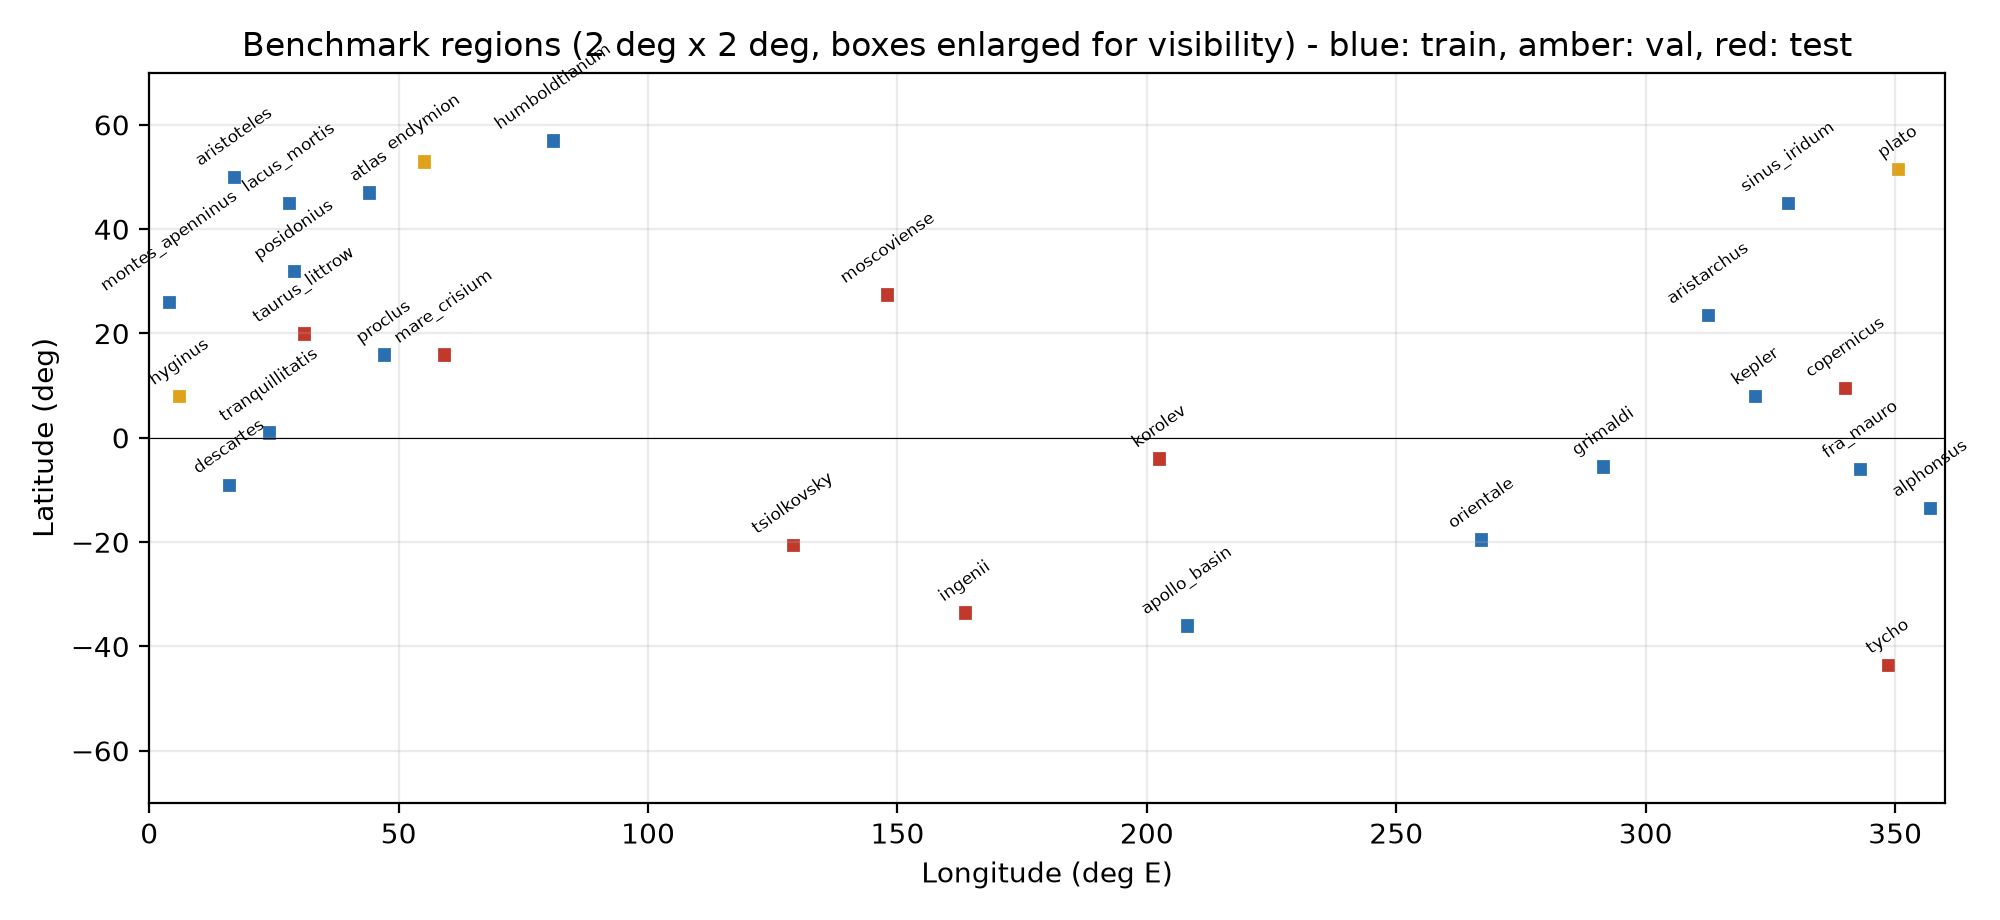
\includegraphics[width=0.9\linewidth]{region_map.png}
\caption{Geographic coverage and split assignment.}
\end{figure}
\begin{figure}[H]\centering
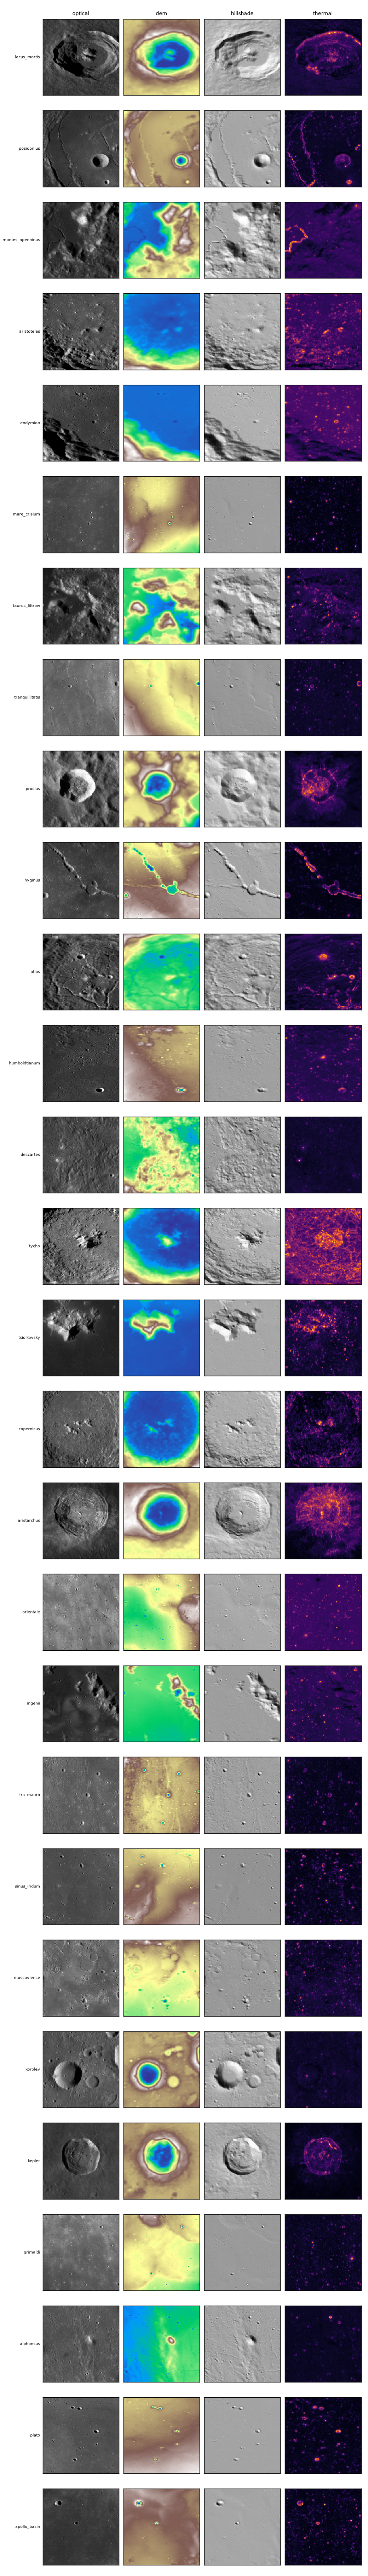
\includegraphics[height=0.85\textheight]{region_montage.png}
\caption{Optical, elevation, hillshade and thermal layers for every region.}
\label{fig:montage}
\end{figure}

\section{Alignment Quality}
Alignment is exact by georeferencing and common-grid construction. As an
independent check we shift the optical layer relative to the terrain layer by
up to $\pm5$~px and measure normalized cross-correlation between optical
gradient magnitude and slope (Table~\ref{tab:reg}). The best-agreement shift is always within the $\pm5$~px search window, is
at most 3~px in 25 of 28 regions, and the east--west component $dx$ is positive
in 16 regions, negative in 10 and zero in 2: the sign is not consistent, with a
mild preponderance of positive values that may reflect the illumination
asymmetry discussed below. Zero shift is
close to the best in most regions but is the maximum in only one
(\texttt{alphonsus}); \texttt{proclus}, whose bright ray system dominates optical
gradients, has the weakest correlation (0.18 at zero shift) and its best shift
lies at the window edge. Because albedo-edge asymmetry from the WAC sun angle
biases this statistic, we treat it as a consistency check and not as evidence
of residual misregistration; it cannot certify sub-pixel accuracy.

\paragraph{Crater-based check.}
A second check does not use slope or gradient correlation. For craters of
2--30~km diameter in the Robbins database \cite{robbins2019craters} that lie
fully inside a region, we estimate each crater's centre separately in every
layer as the position (within $\pm6$~px of the catalogued centre) that
maximises radial symmetry, i.e.\ the fraction of variance within 1.3 radii
explained by the azimuthal mean profile, and report the median offset relative
to the elevation layer. The catalogue only places the search window.
In 106 craters from 23 regions, the thermal-minus-elevation median offset is
$(dy,dx)=(-0.02,-0.02)$~px with 95\% bootstrap intervals of
$[-0.20,0.14]$ and $[-0.37,0.25]$~px (66 craters pass the symmetry threshold
in both layers). For the optical layer the raw brightness gives a median
$dx=1.06$~px with an interval of $[-1.8,3.1]$~px: the WAC mosaic's fixed sun
direction makes brightness asymmetric across a crater, so this estimate is
dominated by illumination. Using the optical gradient magnitude, whose rim
edges appear on both sides of a crater, gives $(0.15, 0.55)$~px with intervals
$[-0.05,0.35]$ and $[-0.18,1.34]$~px (73 craters). The gradient-magnitude
variant was introduced after seeing the raw-brightness bias. Single-crater
offsets are noisy (median absolute deviation about 1--2~px), so these results
bound a systematic offset between layers to about one pixel (237~m) or less;
they do not demonstrate sub-pixel registration, and the number of suitable
craters per region is too small for per-region conclusions.
\begin{table}[H]\centering\small
\begin{tabular}{lrrrrrr}
\toprule
region & ncc\_zero\_shift & ncc\_best & best\_dy & best\_dx & best\_shift\_m & zero\_rank\_of\_121 \\
\midrule
lacus\_mortis & 0.32 & 0.38 & -3 & 1 & 749.15 & 81 \\
posidonius & 0.52 & 0.57 & 0 & 3 & 710.70 & 42 \\
montes\_apenninus & 0.42 & 0.48 & 1 & -3 & 749.15 & 71 \\
aristoteles & 0.51 & 0.57 & 1 & -2 & 529.73 & 40 \\
endymion & 0.60 & 0.63 & 0 & 2 & 473.80 & 22 \\
mare\_crisium & 0.52 & 0.56 & 0 & 1 & 236.90 & 5 \\
taurus\_littrow & 0.40 & 0.45 & 1 & -2 & 529.73 & 24 \\
tranquillitatis & 0.58 & 0.60 & 0 & 2 & 473.80 & 4 \\
proclus & 0.18 & 0.28 & -1 & 5 & 1207.96 & 120 \\
hyginus & 0.63 & 0.70 & 0 & 2 & 473.80 & 15 \\
atlas & 0.20 & 0.30 & -1 & 3 & 749.15 & 79 \\
humboldtianum & 0.57 & 0.60 & 0 & 2 & 473.80 & 7 \\
descartes & 0.38 & 0.49 & 0 & -2 & 473.80 & 21 \\
tycho & 0.42 & 0.48 & 1 & 2 & 529.73 & 34 \\
tsiolkovsky & 0.61 & 0.67 & 0 & -4 & 947.60 & 70 \\
copernicus & 0.52 & 0.56 & 1 & -1 & 335.03 & 11 \\
aristarchus & 0.39 & 0.41 & 1 & 3 & 749.15 & 42 \\
orientale & 0.50 & 0.53 & 0 & 2 & 473.80 & 5 \\
ingenii & 0.61 & 0.65 & 0 & -3 & 710.70 & 32 \\
fra\_mauro & 0.63 & 0.66 & 1 & 2 & 529.73 & 6 \\
sinus\_iridum & 0.62 & 0.69 & 0 & 2 & 473.80 & 5 \\
moscoviense & 0.64 & 0.66 & 0 & -1 & 236.90 & 7 \\
korolev & 0.32 & 0.41 & 1 & -3 & 749.15 & 61 \\
kepler & 0.49 & 0.55 & 0 & 4 & 947.60 & 43 \\
grimaldi & 0.47 & 0.47 & 1 & 0 & 236.90 & 2 \\
alphonsus & 0.57 & 0.57 & 0 & 0 & 0.00 & 1 \\
plato & 0.59 & 0.72 & 0 & 2 & 473.80 & 12 \\
apollo\_basin & 0.64 & 0.75 & 1 & -2 & 529.73 & 16 \\
\bottomrule
\end{tabular}

\caption{Cross-modal shift check per region (1~px $\approx$ 237~m).}\label{tab:reg}
\end{table}

\section{Tasks, Splits and Baselines}
\paragraph{Splits.}
By region, never by tile (neighbouring tiles share terrain and illumination).
Test regions: \texttt{taurus\_littrow}, \texttt{mare\_crisium}, \texttt{tycho},
\texttt{tsiolkovsky}, \texttt{copernicus}, \texttt{ingenii},
\texttt{moscoviense}, \texttt{korolev}. Validation: \texttt{hyginus},
\texttt{endymion}, \texttt{plato}. The remaining seventeen regions are used for
training. Leave-one-region-out results
complement the fixed split.
\paragraph{Tasks.}
(1) \emph{Thermal prediction}: Diviner midnight temperature from optical
and/or terrain inputs. (2) \emph{Slope estimation}: slope from optical only.
\paragraph{Metrics.}
RMSE, MAE, $R^2$ computed per test region then averaged, and \emph{anomaly}
$R^2$ computed after subtracting each tile's mean from prediction and target.
Absolute $R^2$ is dominated by between-region offsets and can be strongly
negative; anomaly $R^2$ measures whether within-tile spatial structure is
recovered.
\paragraph{Baselines.}
Train mean; latitude-only quadratic ridge (thermal); ridge and
histogram-gradient-boosting on multi-scale pixel features; a small dilated
CNN with early stopping on the validation regions. Mean $\pm$ std over seeds.

\section{Results}
\begin{table}[H]\centering\small
\begin{tabular}{llllll}
\toprule
Inputs & Model & RMSE & MAE & R2 & Anomaly R2 \\
\midrule
- & mean & 7.595 & 5.982 & -1.481 & -0.000 \\
latitude only & latitude & 8.171 & 6.704 & -1.970 & 0.000 \\
optical & ridge & 7.108 & 5.500 & -1.250 & -0.186 \\
optical & hist\_gb & 6.672 $\pm$ 0.006 & 4.998 $\pm$ 0.006 & -1.759 $\pm$ 0.026 & -0.895 $\pm$ 0.029 \\
optical & cnn & 5.784 $\pm$ 0.107 & 4.265 $\pm$ 0.070 & -1.389 $\pm$ 0.402 & -0.562 $\pm$ 0.229 \\
terrain & ridge & 7.417 & 5.995 & -2.280 & -0.888 \\
terrain & hist\_gb & 7.559 $\pm$ 0.010 & 6.044 $\pm$ 0.009 & -2.649 $\pm$ 0.015 & -1.270 $\pm$ 0.015 \\
terrain & cnn & 7.690 $\pm$ 0.187 & 6.186 $\pm$ 0.148 & -3.508 $\pm$ 0.399 & -1.526 $\pm$ 0.364 \\
optical+terrain & ridge & 7.193 & 5.740 & -2.027 & -0.802 \\
optical+terrain & hist\_gb & 6.835 $\pm$ 0.029 & 5.214 $\pm$ 0.021 & -3.373 $\pm$ 0.142 & -2.076 $\pm$ 0.142 \\
optical+terrain & cnn & 6.595 $\pm$ 0.067 & 4.825 $\pm$ 0.079 & -4.232 $\pm$ 0.300 & -2.848 $\pm$ 0.163 \\
optical+terrain [LORO] & hist\_gb & 6.266 & 4.861 & -3.157 & -1.536 \\
optical+terrain [LORO] & mean & 6.487 & 5.071 & -1.471 & -0.000 \\
\bottomrule
\end{tabular}

\caption{Thermal prediction on held-out regions (K).}\label{tab:thermal}
\end{table}
\begin{table}[H]\centering\small
\begin{tabular}{llllll}
\toprule
Inputs & Model & RMSE & MAE & R2 & Anomaly R2 \\
\midrule
- & mean & 6.773 & 4.967 & -1.589 & -0.000 \\
optical & ridge & 5.798 & 4.281 & -0.041 & 0.089 \\
optical & hist\_gb & 4.831 $\pm$ 0.003 & 3.603 $\pm$ 0.004 & 0.262 $\pm$ 0.003 & 0.294 $\pm$ 0.003 \\
optical & cnn & 4.208 $\pm$ 0.106 & 2.884 $\pm$ 0.049 & 0.457 $\pm$ 0.019 & 0.428 $\pm$ 0.009 \\
optical [LORO] & hist\_gb & 4.114 & 2.976 & 0.121 & 0.239 \\
optical [LORO] & mean & 6.026 & 4.653 & -2.369 & -0.000 \\
\bottomrule
\end{tabular}

\caption{Slope estimation from optical imagery (deg).}\label{tab:slope}
\end{table}
\paragraph{Thermal prediction.}
On the eight held-out regions the train-mean predictor reaches 7.59~K RMSE and
the latitude-only model is worse (8.17~K), so latitude alone does not explain
midnight temperature across these terrains. The CNN reaches $5.78\pm0.11$~K
from optical inputs, $7.69\pm0.19$~K from terrain alone (no better than the
train mean) and $6.60\pm0.07$~K from both, so adding terrain to the optical
input does not help the CNN; gradient boosting shows the same ordering
(6.67~K optical, 6.83~K both, 7.56~K terrain alone). Optical appearance is
therefore the most informative input for midnight temperature here. Much of the
gain comes from regions far from the training distribution: for \texttt{tycho}
the optical-input CNN lowers RMSE from 23.5 to 12.3~K and for
\texttt{copernicus} from 12.0 to 7.3~K, while \texttt{tsiolkovsky} improves
less (11.4 to 9.9~K). On the five low-variance regions
\texttt{mare\_crisium}, \texttt{taurus\_littrow}, \texttt{ingenii},
\texttt{moscoviense} and \texttt{korolev} the optical CNN is worse than the
mean (for example 4.0 vs 3.4~K on \texttt{mare\_crisium} and 3.5 vs 3.1~K on
\texttt{taurus\_littrow}), because it predicts regional offsets that are wrong
there. Anomaly $R^2$ is not positive for any learned thermal model (Ridge
$-0.19$ to $-0.89$, boosted trees $-0.90$ to $-2.08$, CNN $-0.56$ to $-2.85$;
the latitude-only model is $\approx 0$ by construction): on unseen regions these
baselines predict \emph{region-level} thermal offsets but do not recover
within-tile thermal structure. The low-variance \texttt{korolev} region
contributes the most negative values. This is the main open problem the
benchmark exposes.
Leave-one-region-out agrees: boosted trees on optical and terrain reach
6.27~K versus 6.49~K for the train mean (a gain of 3\%) with anomaly
$R^2=-1.54$.

\paragraph{Slope estimation.}
Estimating slope from optical imagery alone is learnable across regions: the
CNN reaches $4.21\pm0.11^\circ$ versus $6.77^\circ$ for the train mean, with
anomaly $R^2=0.43\pm0.01$ (boosted trees $4.83^\circ$, 0.29; ridge
$5.80^\circ$, 0.09). Leave-one-region-out with boosted trees gives
$4.11^\circ$ versus $6.03^\circ$ (anomaly $R^2=0.24$). The largest structural
gains of the CNN are on \texttt{ingenii} and \texttt{tsiolkovsky} (anomaly
$R^2=0.54$ each), followed by \texttt{moscoviense} (0.48) and \texttt{korolev}
(0.47); \texttt{tycho} is lowest (0.26), followed by \texttt{copernicus}
(0.36) and \texttt{taurus\_littrow} (0.38).

\paragraph{Take-aways and caveats.}
(i) The benchmark separates models that merely fit regional offsets from those
that capture spatial structure, a distinction absolute $R^2$ hides. (ii) The
baselines are deliberately simple; the CNN's seed-to-seed standard deviation
($\approx$0.1~K on thermal) is as large as some differences between input
variants, and the number of held-out regions (eight) is small, so
per-region results should be read individually. (iii) Leave-one-region-out
rows use different test sets from the fixed split and are not directly
comparable with it; each is compared with its own train-mean reference.

\section{Limitations}
The pixel-level thermal data are a single local-time (midnight) product (the
diurnal curve is tile-level only); the common grid is
coarser than native WAC; 28 boxes of $\sim$60~km do not represent the whole
Moon; illumination differs across layers; WAC nodata and rare gap pixels must
be masked (see dataset card). Baselines are intentionally simple and are not
tuned beyond validation-based early stopping.

\section{Reproducibility and Ethics}
Code, region registry, splits and tables are generated from public PDS data
with a single command per stage (\texttt{run\_pipeline.py},
\texttt{src.experiments.*}); offline tests are in \texttt{tests/}. Data are
NASA open data; no human subjects or personal data are involved.
\TODO{license statement, archive DOI (Zenodo/Hugging Face), code URL.}

\bibliographystyle{plain}
\bibliography{refs}
\end{document}
